%----------------------------------------------------------------------------   
\chapter{Használt eszközök bemutatása}
%---------------------------------------------------------------------------- 

\section{Híváshoz használt protokollok}

\subsection{RTP \& RTCP}

Az RTP protokoll használatával valós időben lehet hang, videó vagy egyéb multimédiás 
információkat szállítani egy-egy felhasználó között. A valós idejű továbbítás mellett
információkat szolgáltat arról, hogy a csomag tartalma milyen kódolást használ, 
sorszámozza a csomagokat, ellátja őket időbélyeggel és lehetővé teszi szállítási folyamat
monitorozását. Az alkalmazások általában UDP felett használják az RTP-t így ki lehet
használni az UDP által nyújtott előnyöket. Ez viszont nem azt jelenti, hogy az RTP
csak UDP-vel tud működni, mert elméletileg minden UDP-hez hasonló protokoll tudja kezelni
az RTP-t.

Fontos megjegyezni, hogy az RTP nem szolgáltat semmilyen mechanizmust, ami biztosítaná,
hogy a csomagok időben megérkeznek így QoS-t (Quality of Service) sem garantál. Ezen kívül
az RTP nem garantálja, hogy a csomagok egyáltalán megérkeznek, nem akadályozza meg, hogy a 
csomag soron kívül érkezzenek és nem ellenőrzi, hogy a használt hálózat megbízható és az
sorban szállítja le csomagokat. A fogadó alkalmazás feladata, hogy csomagokat sorba rendezze
a bennük megtalálható sorszám alapján. \\

Ahhoz, hogy bővebb információt lehessen kapni az RTP folyam állapotáról periodikusan a 
felek küldenek egymásnak RTCP csomagokat. Ezek a csomagok szintén UDP felett működnek,
mivel ugyanazokra a funkcionalitásokra van szükség ebben az esetben is. Fontos megjegyezni
még azt is, hogy az RTP csomagok mindig páros portra érkeznek, míg az RTCP mindig az eggyel
nagyobb portot fogja használ így az mindig páratlan lesz.

Fontos, hogy az RTCP csomagoknak számunkra két fő típusa van, amiket jelentéseknek hívnak.
Ezek a jelentések tartalmazzák az aktuális RTP folyamról alkotott információk halmazát. Egy
ilyen jelentést mindig a küldő készít és egyet a fogadó. Viszont ez a kettő jelentés nem azonos
mezőket tartalmaznak, mert a fogadó jelentésben számításba van véve a küldő jelentéseknek 
a tartalma és ideje. Így van küldő és fogadó jelentés is, amiket a hívásban résztvevő felek 
mindegyike periodikusan előállít. Ez a periodicitás attól függ, hogy a hálózat mekkora 
sávszélességgel rendelkezik, ha nagyobb a sávszélesség, akkor több jelentés fog születni és
jobb képet lehet kapni arról, hogy milyen RTP folyam minősége, míg alacsonyabbnál kevesebb
RTCP csomag kerül kiküldésre. 

A \cite{RFC3550} leírásában szereplő RTCP csomagok leírása alapján a fontosabb részei a
küldő és fogadó jelentésnek. Kezdve a küldőével: 

\begin{itemize}
	\item SSRC (Synchronization source), amivel jelöli, hogy kitől származik egy a jelentés.
	\item A jelentés küldésének idejét, ami a küldő órájának pontos ideje. Körülfordulási
	idő mérésére használható. 
	\item RTP csomagokban használt időbélyeg. 
	\item A küldő által elküldött csomagok száma és azok mérete.
\end{itemize}

Míg a fogadó jelentés az alábbi részekkel rendelkezik:

\begin{itemize}
	\item SSRC.
	\item Töredékveszteség, ami az előző küldő és fogadó jelentés óta elvesztett RTP csomagok
	száma van jelölve.
	\item Az összes elveszett csomag száma. 
	\item Legmagasabb kapott sorszám. 
	\item A csomag küldési időpontjától az érkezés idejéig eltelt idő, ami a jitter. Ez az érték
	minden fogadó jelentés során újra van számolva a két jelentés között érkezett csomagok 
	alapján.
	\item Az utolsó kapott küldő jelentés ideje és az azóta eltelt idő.  
\end{itemize}

\subsection{SIP}

A SIP egy olyan alkalmazás rétegben működő viszonykezdeményező protokoll, amivel 
létrehozni, módosítani és törölni lehet kapcsolatokat felek között. Ezek a kapcsolatok 
általában az internet telefonálás vagy multimédiás forgalom lebonyolítását valósítják meg. 

A SIP működése során fontos, hogy a felhasználók azonosíthatóak legyenek valamilyen
paraméter szerint, amihez sok esetben nem elegendő szimplán az IP cím. Egy 
SIP kliens egyéniségét a SIP URI (Uniform Resource Identifier) fogja megadni, ami
a  felhasználó nevéből és a SIP szerver által meghatározott tartománynévből áll.
Ez a cím úgy néz ki, mint egy átlagos email cím azzal a különbséggel, hogy az 
elején szerepel a \textit{sip:} szó. Egy példa arra, hogyan néz ki egy ilyen cím: 
sip:peter@tartomany.com. Így ha az egyik kliens hívást kezdeményez Péter felé,
akkor ezzel a címmel pontosan meglehet határozni az elhelyezkedését. 

Működése nagyban hasonlít a HTTP (HyperText Transfer Protocol) kommunikációhoz, ahol 
a kliens bizonyos kéréseket küld a szerver felé, amire választ kap. A \cite{RFC3261}-ben
olvasható több parancs közül a szakdolgozat szempontjából a következők fontosabbak: 

\begin{itemize}
	\item \textbf{INVITE}: Új kapcsolat létesítése.
	\item \textbf{ACK}: INVITE üzenet elfogadását jelzi. 
	\item \textbf{BYE}: Kapcsolat befejezése. 
	\item \textbf{REGISTER}: Felhasználó regisztrálása a SIP szerverre. 
\end{itemize}

A SIP protokoll szerves része az SDP (Session Description Protocol), amivel a multimédia
folyamatok kiépítésénél van szükséges. Ugyanis ebben a protokollban lehet megadni,
hogy milyen média kódolásokat támogatnak a hívásban résztvevő felek és mely
portokon várják a médiaforgalmat. Ezeken az információkon kívül még rengeteg 
más hasznos információt is lehet közölni ezekben az üzenetekben, viszont a 
szakdolgozat szempontjából csak a támogatott kódolás és a kapcsolat leírására
szolgáló paraméter a fontos.

\section{Kubernetes}

A Kubernetes egy nyílt forráskódú konténer kezelő platform, amivel automatizálni
lehet a legtöbb feladatot, ami a fejlesztés, karbantartás vagy skálázással 
kapcsolatos. A Google fejlesztette eredetileg, de jelenleg a Cloud Native
Computing Foundation - CNCF vette át a karbantartását. 

Kubernetes fürtöt létrehozhatunk lokálisan a saját szerveren is vagy felhőben,
ami lehet publikus, privát vagy hibrid hozzáférésű is. Viszont azt figyelembe 
kell venni, hogy egy Kubernetes fürtöt nem egyszerű kiépíteni lokálisan, 
szóval ha nem szükséges, akkor lehet használni felhőszolgáltatók Kubernetes 
motorjait, mint az Amazon AKS, Linode LKE vagy a Google GKE szolgáltatása.
Ilyenkor az általunk beállított paraméterekkel létrejön egy teljes fürt, amit
tudunk menedzselni.

\subsection{Felépítése}

\begin{figure}[!ht]
	\centering
	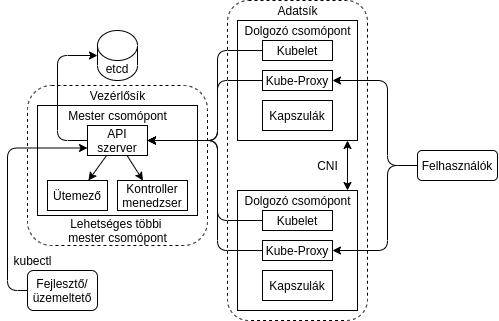
\includegraphics[width=1\textwidth, keepaspectratio]{figures/k8s_architecture.png}
	\caption{Kubernetes fürt felépítése}
	\label{fig:achitecture}
\end{figure}

Egy Kubernetes fürt kettő részből áll egy vezérlő- és egy adatsíkból, ahol a 
vezérlősíkban szereplő mester csomópontok tudják vezérleni az adatsíkban 
lévő dolgozó csomópontokat és a fejlesztők vagy üzemeltetők a mester által
hirdetett API-n (Application Programming Interface) keresztül képesek parancsokat
kiadni. Míg a dolgozó csomópontokon futó alkalmazáshoz a felhasználók csak az 
általuk hirdetett Kube-Proxy segítségével tudnak hozzáférni. 

A kapcsolat mester és dolgozó között az API szerver és a Kubelet kommunikációján
alapul. Ha a fejlesztő szeretne egy új alkalmazást telepíteni a fürtön, akkor
szól az API szervernek, ami majd kiadja a megfelelő parancsokat a Kubelet-nek 
és majd az fogja a konténereket létrehozni. Amiről az API szervert értesítve 
tudja meg a fejlesztő, hogy amit csinált az létrejött.

\subsubsection{Vezérlősík}

A mester csomópont mindig a fő vezérlő egysége a fürtnek, mivel kezeli a 
munkafolyamatokat és irányítja a kommunikációt fürtön belül. A \ref{fig:achitecture}-s ábrán
látható vezérlősík tartalmazhat  több mester csomópontot is a felsorolt 
komponensekkel, amivel lehet biztosítani a fejlesztők számára a folytonos 
elérést. A mester csomópont részei: 

\begin{itemize}
	\item \textbf{etcd}: Egy állandó kulcs-érték alapú adatbázis, ami tárolja 
	a fürt konfigurációs beállításait és a fürt állapotát. Fontos az a rész, 
	hogy ez egy állandó adatbázis, mivel ez a csomóponton fut és nem egy 
	kapszulában.   
	\item \textbf{API szerver}: Egy REST API (Representational State Transfer API) 
	szerver, ami hozzáférést biztosít a fürthöz a fürtön belül és azon kívül is. 
	Egyszerű HTTP üzenetekbe ágyazott JSON (JavaScript Object Notation) konfigurációkkal
	lehet beállítani, hogy mit csináljon a fürtben. De a dolgozó csomópontok is ezen 
	keresztül küldenek frissítést az etcd-be. 
	\item \textbf{Ütemező}: Ez a komponens dönti el, hogy egy új kapszula melyik
	dolgozó csomóponton legyen létrehozva aszerint, hogy van-e megfelelő erőforrás
	az adott csomópontot megvalósító szerveren.
	\item \textbf{Kontroller menedzser}: Egy olyan állandóan futó folyamat ami ellenőri,
	hogy a kapszulák bizonyos esetekben újrainduljanak vagy hogy egy ismétlődő 
	munkafolyamat időnénként lefusson helyesen. Ezt az API szerverrel kommunikálva
	képes megvalósítani. 
\end{itemize}

Mint ahogy a \ref{fig:achitecture}-s ábrán is látszik a fejlesztő vagy üzemeltető alapvetően a \textbf{kubectl}
nevezetű eszközzel képesek kommunikálni az API szerverrel. Ez az eszköz lényegében
megvalósítja a teljese HTTP kommunikációt az API szerverrel szóval sokkal könnyebben 
lehet vele lekérdezni információkat vagy új erőforrásokat létrehozni. 

\subsubsection{Adatsík}

Az adatsíkon futnak az úgynevezett dolgozók, amik igazából különálló szerverek,
amik rendelkeznek a \ref{fig:achitecture}-s ábrán szereplő komponensekkel és képesek futtatni 
valamilyen konténer kezelő alakalmázást, mint például a Docker. Ami régebben az 
alapértelmezett konténer kezelője volt a Kubernetes-nek, de 2021-ben már nem 
követeli meg és bármilyen másik konténer kezelőt is be lehet állítani alapértelmezettnek.
A fontosabb elemei az adatsíknak:

\begin{itemize}
	\item \textbf{Kubelet}: Felelős az egyes csomópontok futási állapotáért biztosítva, 
	hogy a csomóponton lévő összes konténer egészséges legyen. Gondoskodik az alkalmazás
	konténereinek indításáról, leállításáról és karbantartásáról, amelyek kapszulákba 
	vannak rendezve a vezérlősík utasítása szerint
	\item \textbf{Kube-Proxy}: Egy proxy és terheléselosztó megvalósítása, ami biztosítja
	a szolgáltatás elérhetőségét más hálózatok számára. Így a feladata az, hogy a beérkező
	forgalmat a megfelelő konténerekhez irányítsa, amit különböző paraméterek szerint képes
	megvalósítani.
	\item \textbf{Kapszulák}: A legkisebb menedzselhető egységek amiket lehet telepíteni
	Kubernetes alatt. Egy kapszula több konténernek a csoportja, amik osztoznak a tárolási
	és hálózati erőforrásokon és specifikálja, hogy a konténerek hogyan fussanak. 
	\item \textbf{CNI (Container Network Interface)}: A kapszulák hálózati interfészeinek
	a beállítására lehet használni. Így lehet specifikálni, hogy a kapszulák között 
	milyen hálózatot használva legyen továbbítva a forgalom. 
\end{itemize}

\subsection{Erőforrások}

A \ref{fig:achitecture} leírt architektúra csak az alapjai a Kubernetesnek, viszont ezen kívül
még rengeteg olyan erőforrással is rendelkezik, amik lehetővé teszik a konténerek
menedzselésének egy új szintjét.

A következőkben leírom, hogy a projekt szempontjából mely erőforrások lesznek még
lényegesebbek. Viszont rengeteg olyan erőforrásról lehet többet olvasni \cite{kubeAPI}
amiket a Kubernetes segítségével lehet létrehozni.   

\begin{itemize}
	\item \textbf{Replikációs vezérlő}: Biztosítja, hogy egy meghatározott számú 
	kapszula replika fusson egyszerre, amivel biztosítja az alkalmazás magas szintű
	elérhetőségét. Ami azt eredményezi, ha túl sok kapszula fut, de nem kellene nekik,
	akkor törli azokat vagy, ha túl kevés, akkor újakat hoz létre. Mindazonáltal, 
	ha egy kapszula maga vagy az egyik konténere hibát eredményez, akkor újraindítja
	a benne lévő konténer vagy a teljes kapszulát. 
	\item \textbf{Telepítő (Deployment}): Leír egy elvárt állapotot, ami alapján a
	replikációs vezérlő tudja, hogy milyen specifikáció szerint kell az új kapszulákat
	létrehozni vagy a létrehozandó kapszulák számát. 
	\item \textbf{DaemonSet}: Biztosítja, hogy az összes vagy néhány csomópont 
	futtassa egy meghatározott kapszula másolatát. Így, ha egy új dolgozó csomópont 
	csatlakozik a fürthöz, akkor ez a kapszula automatikusan megjelenik rajta. Tipikusan
	valamilyen tárolási vagy monitorozási feladatot ellátó kapszulát szokás ilyen
	módon létrehozni, de a későbbiekben látni fogjuk, hogy az l7mp ugyan ezzel a 
	módszerrel hozza létre a bejárati pontokat a csomópontokon.
	\item \textbf{DNS (Domain Name System)}: Tárolja a fürtben szereplő minden kapszula 
	és szolgáltatás IP címét illetve a hozzájuk kapcsolódó tartomány nevüket is.  
	\item \textbf{Szolgáltatás}: Egy absztrakt módja az alkalmazást futtató kapszulák
	kiexponálásának a hálózaton keresztül. Mivel a kapszulák halandóak így nem mindig
	ugyanazon a címen lesznek elérhetőek a rajtuk futtatott alkalmazások. A megoldás
	erre, ha egy címke alapján hozzárendeljük őket egy szolgáltatáshoz, ami mindig 
	elérhető lesz ugyanazon a címen és képes elosztani a forgalmat több kapszula között.
	A forgalomirányítást a szolgáltatások a Kubernetes DNS szolgáltatása miatt tudják 
	megvalósítani. Mivel minden kapszula rendelkezik egy tartománynévvel és ez a Kubernetes
	DNS leírójában szerepel egy hozzá tartozó IP címmel.
	\item \textbf{Bejárat (Ingress gateway)}: Egy olyan API objektum, ami kezeli a 
	külső hozzáférést különböző szolgáltatásokhoz a fürtön belül. Így a bejövő forgalmat
	könnyen lehet szűrni illetve típusától tartalmától függően más és más szolgáltatásokhoz
	lehet irányítani. 
	\item \textbf{Egyéni erőforrás definíció (Custorm Resource Definition)}: A 
	Kubernetes API egy olyan kiterjesztése melynek során új fajta erőforrás definíciókat
	lehet definiálni. Így bővítve a Kurbenetes funkcionalitását.
	\item \textbf{Pótkocsi (Sidecar)}: Mivel egy kapszula több konténert is tartalmazhat
	és ezek a konténerek megosztják a hálózatukat így létre lehet hozni egy olyan konténert
	ami csak a hálózati forgalom kezelésével foglalkozik. Így könnyen lehet szűrni, hogy
	milyen forgalom juthat csak el az alkalmazást futtató konténerhez. Mivel elsőnek 
	mindig ezen pótkocsin fog áthaladni a forgalom majd lokális hálózaton átadja az
	alkalmazásnak. Ezek a pótkocsik általában valamilyen proxyk szoktak lenni. 
	\item \textbf{RBAC (Role-based access controll)}: Ha több fejlesztő vagy üzemeltető
	fér hozzá az API szerverhez, akkor egyénenként meglehet mondani, hogy kinek milyen 
	művelet végrehajtására van joga. Így például korlátozható, hogy ki képes új
	erőforrásokat létrehozni. Viszont a felhasználók mögött sokszor nem egy élő 
	személy van, hanem egy alkalmazáshoz van hozzárendelve. Így az alkalmazás esetlegesen
	képes a fürtön belülről erőforrásokat kezelni.
	\item \textbf{Operátor}: Olyan bővítések, amikkel egyéni erőforrások menedzselése
	valósítható meg. De emellett különböző eseményeknél lehet bizonyos folyamatokat 
	elindítani. Példának okáért, ha egy kapszula létrejön, akkor beállíthatjuk, hogy
	rendelkezzen mindig egy adott címkével.
	\item \textbf{Szolgáltatás háló (Service Mesh)}: Meghatározza, hogy a fürt 
	különböző részei hogyan kommunikáljanak egymással. Ezt általában a pótkocsikkal és 
	egy operátorral valósítják meg. A pótkocsik fognak rendelkezni azokkal a beállításokkal,
	hogy milyen a mellettük futó konténer milyen forgalmat fogadhat és az operátor 
	fog arról gondoskodni, hogy a résztvevő kapszulák pótkocsijai mindig a megfelelő
	beállításokkal jöjjenek létre.
\end{itemize}

\section{L7mp}

Az l7mp egy kísérleti alkalmazásréteg és több protokollt támogató szolgáltatás- 
proxy és háló keretrendszer. A hangsúly a több protokoll támogatásán van, amely
lehetővé teszi, hogy sok szállítási és alkalmazásréteg béli protokollt 
natívan támogasson és ne csak a szokásos TCP/HTTP (Transmission Control Protocol) 
protokollokat. Lehetővé teszik emellett még a protokollok közötti konvertálást is 
így könnyen lehet alkalmazási rétegű protokollokat konvertálni szállításiba és vissza is.

Az l7mp, egy vezérlő- és adatsíkból áll, mint a Kubernetes. Ahol az adatsíkot 
az l7mp proxy valósítja meg. Míg a vezérlőt egy operátor, ami képes kezelni 
az l7mp proxy példányokat. 

Ha egy másik szoftverhez kellene hasonlítani az l7mp-t, akkor leginkább az 
Envoy-hoz lehetne, hiszen felépítésében nagyon hasonló elemeket használ, mint
az Envoy. Így akinek van valamilyen tapasztalata az Envoy-l az könnyen kiismeri
magát az l7mp-vel is.  \\

Szeretném megemlíteni, hogy Dr. Rétvári Gábor Ferenc vezetésével a nyári
gyakorlati időm alatt és jelenlegi munkámként ennek a szoftvernek a tesztelésével 
illetve fejlesztésével foglalkozom. 

\subsection{L7mp, mint proxy}

Az l7mp egy olyan programozható proxy, ami nagyon hasonlóan működik, mint az Envoy, ami 
egy széleskörűen használt leginkább alkalmazási réteget támogató proxy. A különbség
az l7mp és az Envoy között, hogy az l7mp a szállítási réteg protokolljait 
támogatja jobban míg az Envoy inkább az alkalmazásréteg protokolljait képes jobban kezelni.
Emellett az l7mp képes protokollok közötti átalakítást végezni, ami sok esetben nagyon
jól tud jönni. Ez a funkcionalitás az architektúra leírása után fog jobban 
megmutatkozni.

A proxy egy magas szintű keretrendszerben íródott, ezért nagyon egyszerűen 
lehet új funkciókkal bővíteni. Ez a keretrendszer a Node.js, ami egy JavaScript
futtató környezet a Google Chrome V8-s JavaScript motorjára építve. Ez szerencsés 
választás a már említett egyszerű bővíthetőség miatt, de  amiatt is, hogy
könnyen lehet vele aszinkron módon programozni. Így nincsenek blokkoló műveletek,
amiket külön szálon kellene futtatni. De behozza azt a hátrányt is, hogy a 
JavaScript miatt lassabb az l7mp, mint az Envoy, ami C++-ban van írva. 

A lassúság kiküszöbölésére jelenleg vannak munkálatok, amik elsősorban azt 
célozzák meg hogy a csomagok feldolgozása nem a felhasználói névtérben kerüljenek
végrehajtásra, hanem kernel szinten. Így a csomagoknak nem kell fájlleírókon 
keresztül eljutnia az l7mp-hez, hanem az l7mp konfigurálása folyamán lehetne
olyan \textit{iptables} szabályokat létrehozni, amik megoldják a csomagok továbbítását
anélkül, hogy írni vagy olvasni kellene a fajleírókat. Az iptables egy olyan 
kernel szintű program, amely lehetővé teszi a csomagok feldolgozását és továbbítását
a kernelben. \\

Az l7mp proxy használható szimplán Node.js-l indítva, mivel elérhető az NPM (Node 
Package Manager) tárolóban. Az indítása a \ref{lst:nodeL7mp} paranccsal történik: 

\begin{lstlisting}[caption=L7mp indítása Node.js segítségével, label=lst:nodeL7mp]
	node l7mp-proxy.js -c config/l7mp-minimal.yaml -l warn -s
\end{lstlisting}

Ami a minimális l7mp konfigurációval és a figyelmeztetési naplózási szinten fogja
elindítani az l7mp proxyt. A minimális konfiguráció létre fog hozni egy REST API
szervert, amin keresztül a későbbiekben újabb l7mp beállításokat lehet megadni.

Ezen felül a Docker-t is támogatja, ami alapértelmezetten a \ref{lst:nodeL7mp} parancsot fogja
egy konténerben futtatni.

\subsubsection{Felépítése}

Mivel az l7mp tervezése során az Envoy volt a minta, így főbb elemei között szerepelnek
ugyanolyan vagy hasonló elemek. A legfontosabb építőkockái az l7mp-nek 
felsorolásra és kifejtésre kerülnek alább: 

\begin{itemize}
	\item \textbf{Munkamenet (Session)}: Munkameneteket nem lehet manuálisan létrehozni,
	mivel ezek akkor generálódnak, amikor egy figyelő forgalmat kap és azt 
	továbbítja valamerre. Egy munkamenet információkat tartalmaz a csomagok típusáról,
	forrás címéről és céljáról. Emellett a munkamenet objektum felelős azért is, hogy a
	a benne lévő objektumok tudják, hogy a hozzájuk beérkező csomagokat fel kell dolgozniuk. 
	\item \textbf{Figyelő (Listener)}: Definiálni lehet vele egy cím és port párost, hogy
	adott protokollal rendelkező csomagokra figyeljen és dolgozza fel őket. A feldolgozás
	alatt azt a folyamatot kell érteni, hogy meghatározza mely fürthöz kerüljön a csomag,
	szűri a bejövő csomagokat valamilyen paraméter alapján, ha lehet. Ez általában 
	a csomagok fejlécében szereplő információk, vagy a munkamenetben megtalálható bármilyen
	érték alapján történhet. 
	\item \textbf{Fürt (Cluster)}: A végpontok egy gyűjteménye, ami képes forgalmat elosztani
	közöttük. Az elosztás történhet nagyon egyszerűen, amikor mindig egy lista élén álló
	végpont kapja a forgalmat, de történhet HashRing módszerrel is. Amikor egy kulcs szerint
	történik a végpont kiválasztása. Ez egy hasznos funkció, mivel így fix kulcs mellett,
	minden csomag ugyanahhoz végponthoz fog kerülni. 
	\item \textbf{Végpont (Endpoint)}: A csomag végállomása, ami lehet a már a csomagokat
	feldolgozó alkalmazás vagy egy másik figyelő is. Így egész komplex folyamatokat 
	lehet kiépíteni, ha szükség van rá. 
	\item \textbf{Szabály (Rule)}: Szabályokat a figyelőkben lehet létrehozni, amikkel
	belehet állítani, hogy mi legyen a célja a beérkező csomagoknak vagy meglehet vele azt
	is határozni, hogy a fejléc mely paraméterét mire módosítsa. 
	\item \textbf{Útvonal (Route)}: Meghatározza a célt, ami általában egy fürt. Az 
	útvonalak mindig a szabályokon belül vannak, hiszen a szabályok határozzák meg a célt.
	De ezen felül még be lehet azt is állítani, hogy a bejövő csomagok milyen útvonalon 
	jussanak el a fürtig és milyenen vissza. Így a bejövő és kimenő forgalmat teljesen 
	más útvonalon lehet irányítani.
\end{itemize}

A Munkamenet kivételével ezeket az elemeket egy jól definiált API leírás alapján 
könnyedén lehet konfigurálni. Így az l7mp proxy egyszerű HTTP POST üzenetekkel 
beállítható.

\subsubsection{Programozása}

Az l7mp programozása történhet konfigurációs fájlból és REST API hívásokon keresztül
egyaránt. Viszont az l7mp indításához szükség van egy alapkonfigurációra, mivel
anélkül nem fog létrejönni a kontroller figyelő, ami biztosítja az API 
láthatóságát. A \ref{lst:minl7mp} kódrészleten látható, hogyan lehet egy ilyen induló konfigurációt
létrehozni YAML (YAML Ain't Markup Language) fájlal.

\begin{lstlisting}[caption=L7mp minimális konfiguráció, label=lst:minl7mp]
admin:
  log_level: info
  log_file: stdout
  access_log_path: /tmp/admin_access.log
listeners:
- name: controller-listener
	spec: { protocol: HTTP, port: 1234 }
	rules:
    - action:
        route:
          destination:
            name: l7mp-controller
            spec: { protocol: L7mpController }
\end{lstlisting}

A konfigurációt részről részre kifejtem. Az első része, az \textit{admin}, ahol
a naplózás szintjét és helyét lehet meghatározni. A következő szintek vannak:
silly, verbose, info, notice, warn, error, silent. Amik ebben a sorrendben
egyre kevesebb információt naplóznak. A silly kiírja a beérkező csomagok tartalmát
is, míg az info már csak munkafolyamat leírásáig működik.

Az utána következő részben létre jön a controller-listener, ami helyi hálózaton az 
1234 porton hirdeti a REST API pontot, amin keresztül később új konfigurációkat lehet 
megadni. Ehhez egy olyan fürt van használva, amelyhez nem tartozik semmilyen definiált
végpont. Ebben a fürtben egy automatikusan létrejövő API szerepel, amihez beérkeznek 
a figyelőn keresztül a HTTP kérések. 

Ez az API megvalósítja a teljes CRUD-t (Create, Read, Update, Delete) mindent komponensre, 
amivel tudunk létrehozni, olvasni, frissíteni és törölni komponenseket. Minden komponenshez
tartozik egy útvonal, ami így tevődik össze, ha a \ref{lst:minl7mp} példát nézzük: http://127.0.0.1:1234/api/v1/listeners.
Ha erre a címre egy POST üzenetben YAML vagy 
JSON konfigurációt küldünk, akkor az létre fog jönni a proxyn belül. Ami még egy 
hasznos funkció ebben a megvalósításban az a rekurzív lekérés, aminek során egy GET 
üzenettel és az URI paraméterekben a \textbf{recursive=true} beállításával az összes
figyelő definíciója a bennük lévő többi objektummal együtt részletesen megkapható. Kétféle 
API leírás létezik az l7mp-hez egy az önálló proxyhoz \cite{proxy} és egy olyan, amit a 
Kubernetes operátor tud használni \cite{kubeProxy}. Azért létezik kétféle API leírás,
mert az elsőnek létrehozott nem volt teljesen kompatibilis a Kubernetes-sel így 
keletkezett még egy. Jövőbeni tervek között szerepel, hogy csak egy legyen.

\begin{lstlisting}[caption=L7mp konfigurálása API-n keresztül, label=lst:confL7mpAPI]
curl -iX POST --header 'Content-Type:text/x-yaml' --data-binary @- <<EOF  http://localhost:1234/api/v1/listeners
listener:
  spec:
  protocol: WebSocket
  port: 2000
rules:
 - action:
     route:
       destination:
         spec:
           protocol: UDP
           port: 3000
         endpoints:
           - spec:
               address: 127.0.0.1
EOF
\end{lstlisting}

A \ref{lst:confL7mpAPI} hívásban látható, hogy létrehozunk egy figyelőt, ami a 127.0.0.1:2000-s
címen fog WebSocket csomagokat várni, majd azokat UDP-re konvertálva továbbküldeni 
a 127.0.0.1:3000-s címre.

Ezen a példán látszik igazán, hogy milyen egyszerű az l7mp-vel a protokoll konverzió,
mert ilyen rövid beállítással kettő nagyon különböző protokoll között lehet 
átalakítást végezni.

\subsection{L7mp, mint szolgáltatás háló}

A szolgáltatásháló egy olyan keretrendszert foglal magában, amivel a különböző 
mikroszolgáltatások közötti kommunikációt lehet meghatározni. Ezek a szolgáltatások 
konténerek, amik rendelkeznek egy olyan API interfésszel, amin keresztül lehet 
őket programozni. Így a fürtön belül könnyen lehet olyan szolgáltatásokat 
igénybe venni, mint a szolgáltatás felderítés, terhelés elosztás és felügyelhetőség.
Ezeken kívül még rengeteg más funkcióval szokott rendelkezni egy szolgáltatás háló,
de ezeket lehet mondani a legnépszerűbbeknek.

A megvalósításához minden mikroszolgáltatásnak azaz kapszulának rendelkeznie kell 
egy pótkocsival, ami egy adott proxyt fog futtatni. Ez a konténer lesz minden esetben
a belépési pont az alkalmazáshoz. Ezeket a proxykat valahogyan dinamikusan kell tudni
konfigurálni, amit egy operátort segítéségével lehet megtenni. A használt proxyknak 
rendelkezni kell egy olyan interfésszel, amin keresztül lehet őket konfigurálni. 
Az l7mp szolgáltatás háló esetében ezek a proxyk egyértelműen az l7mp sajátja lesz,
aminél az \ref{lst:confL7mpAPI} részben láttuk hogyan lehet egy API interfészt definiálni, amin 
keresztül POST hívásokkal lehet új beállításokat eszközölni.

De ezeket a beállításokat valamilyen módon közölni kell az operátorral, amihez 
szükség van egyéni erőforrásokra. Az l7mp esetében ezek az erőforrások sorra a 
VirtualService, Target és Rule. Ezekben lehet olyan beállításokat megadni, amiket
később az l7mp operátora képes leképezni az l7mp proxyk számára érthető konfigurációra.

\subsubsection{Virtuális szolgáltatás - VirtualService}

Egy virtuális szolgáltatás az absztrakt megvalósítása egy szerveroldali foglalatnak. 
Ami azt jelenti, hogy a benne definiált figyelő a meghatározott kapszulák pótkocsijaiban 
létrefog jönni és kezelni tudja hozzá beérkező forgalmat. 

Egy ilyen erőforrás két fő részből áll, az egyik a kapszulák kiválasztásáért felel míg
a másik azért, hogy milyen definíció kerüljön alkalmazásra a kijelölt kapszulákban.
A kiválasztás mindig valamilyen címke alapján történik, amivel rendelkezik a kapszula. 
Ezt viszont többször lehet használni egy definíción belül, mert meglehet vele határozni,
hogy a figyelő mely kapszulákon jöjjön létre és azt is, hogy a végpontok mely kapszulák 
legyenek. 

A másik fontos része maga a figyelő definíciója, ami nagyon hasonló, mint az l7mp proxy
esetében, de itt már vannak Kubernetes specifikus elemek is, mint a \textit{selector},
amivel a kapszulák kiválasztása történik meg. De ilyen az is, hogy egy Kubernetes 
erőforrásra név szerint lehet hivatkozni, amit majd az operátor feloldva fog az l7mp
proxy konténereknek átadni.

\subsubsection{Target - Cél}

Egy cél definiálásával a kliens oldali foglalatokat lehet meghatározni. Ezeken 
a címeken várja az alkalmazás vagy egy másik figyelő a forgalmat. Mivel egy cél 
lényegében egy fürtöt valósít meg, így ez is a végpontokat tárolja, azzal a különbséggel,
hogy célnál a végpontok a kapszulák, szolgáltatások vagy virtuális szolgáltatások is 
lehetnek. 

A felépítése hasonlóan néz, ki mint a virtuális szolgáltatásoknak szóval van egy 
szelektor, hogy mely pótkocsikon legyen elérhető az adott fürt. Illetve a fürt
definíciója. 

Ebben a definícióban lehet megadni, hogy a milyen protokollú csomagokat fogad, végpontokat
és a terheléselosztás beállításait. A végpontok kiválasztása szintén egy szelektorral
történik, ami a Kubernetes erőforrások címkéi alapján választ. A másik fontos beállítása
a terheléselosztás, ami alapértelmezett esetben, mindig a nyilván tartott kapszulák 
közül az elsőnek fogja irányítani a csomagokat. Viszont be lehet állítani úgy is, hogy
egy a csomag fejlécében lévő mező alapján irányítsa a csomagokat. Ez a megoldás a
HashRing megoldást, használja amivel elérhető, hogy egy kulcs alapján mindig ugyan az
a végpont kapja meg a csomagokat. 

\subsubsection{Rule - Szabály}

Szabályokkal lehet összekötni figyelőket a fürtökkel. De ebben az esetben lehet különálló
CRD-ben szabályokat létrehozni és azokat többször felhasználni. Így átláthatóbbá és 
kontrollálhatóbbá válik a szolgáltatás háló használata. 

Használatukkal lehet szűrni a csomagokat forráscímük, fejlécük és még nagyon sok más 
paraméter szerint. JSON predicate objektumokkal lehet szűrni az csomagokat, amivel 
könnyen lehet komplex szűrési feltételeket meghatározni különböző paraméterek alapján. Ha 
egy csomag megfelel minden kitételnek, akkor a definiált művelet szerint fog tovább 
haladni a csomag. 